\documentclass[11pt]{article}
\usepackage[letterpaper,margin=1in]{geometry}
\usepackage[T1]{fontenc}
\usepackage{times}
\usepackage{graphicx}
\usepackage{booktabs}
\usepackage{natbib}
\usepackage{lineno}
\usepackage{setspace}
\usepackage{hyperref}
\usepackage{amsmath,amssymb}
\linenumbers
\graphicspath{{figures/}}
\hypersetup{colorlinks=true,urlcolor=blue,citecolor=black,linkcolor=black}
\bibliographystyle{genetics}

\title{Benchmarking AgroNT against a DeepSEA-style convolutional network for tissue-averaged gene expression classification in \emph{Arabidopsis thaliana}}
\author{Author names to be completed before submission\\
Department of Plant Sciences, University Name, City, Country\\
Corresponding author: Name. Email: email@university.edu}
\date{}

\begin{document}
\onehalfspacing
\maketitle
\begin{abstract}
Models that classify gene expression from flanking DNA would help plant geneticists annotate uncharacterized genes and prioritize noncoding variants. Compact convolutional networks and plant DNA foundation models are rarely scored on the same genes, labels, and metrics, so the size of any foundation-model gain is hard to read from published suites. We compared a one-dimensional convolutional network in the style of DeepSEA with the one-billion-parameter plant model AgroNT, adapted by low-rank updates, on a tissue-averaged high-versus-low expression task in \emph{Arabidopsis thaliana}. Labels were derived from the Plants Genomic Benchmark Arabidopsis gene-expression sequences by averaging 56 tissue abundances and thresholding at the training-set median. This is a derived binary collapse, not the official multi-tissue regression. On 3,402 held-out Arabidopsis genes, AgroNT reached 86.8\% accuracy and 0.939 area under the receiver operating characteristic curve, versus 75.4\% and 0.842 for the convolutional network (difference 0.097; 95\% confidence interval 0.086--0.108). Mutagenesis placed signal in proximal annotated flanks. Variant-effect ranks differed by architecture: untranslated regions led for the convolutional network, whereas the terminator led for AgroNT. Single-tissue labels agreed with the averaged label for a mean of 92.1\% of genes. On independent rice, maize, tomato, and soybean test sets, the same Arabidopsis checkpoints kept that ranking. Under this locked protocol, low-rank-adapted AgroNT outperforms this convolutional network by a statistically supported margin, with architecture-specific regional variant ranks.
\end{abstract}

\noindent\textbf{Keywords:} gene expression; \emph{Arabidopsis thaliana}; cis-regulatory DNA; DNA language model; convolutional network.

\noindent\textit{G3: Genes, Genomes, Genetics} --- Investigation (review copy with line numbers).













\section{Introduction}

Most of a plant genome is noncoding DNA. Cis-regulatory elements in promoters, 5$'$/3$'$ untranslated regions (UTRs), and terminators determine when, where, and at what level genes are expressed \citep{marand2023}. A sequence-to-expression scorer that reads this code from DNA would support annotation of uncharacterized genes, ranking of noncoding variants, and design of synthetic regulatory DNA \citep{hu2023}.

Convolutional neural networks (CNNs) showed that proximal DNA carries substantial information about transcript abundance. DeepSEA established this for noncoding variant effects \citep{zhou2015}. In plants, \citet{peleke2024} trained interpretable CNNs that classify high-versus-low expression from gene-flanking sequence across four species with $>$80\% accuracy and recovered known transcription-factor motifs by attribution. In parallel, DNA language models pretrained on whole genomes have become general-purpose genomic feature extractors \citep{avsec2021}. AgroNT, a one-billion-parameter transformer pretrained on $\sim$10.5 million sequences from 48 edible plant genomes, reported strong results across the Plants Genomic Benchmark (PGB) \citep{mendoza2024,pgb2024}.

What remains unclear for applied plant genetics is how large the gain of foundation-model fine-tuning is relative to a compact CNN under identical splits, labels, and metrics, and which sequence compartments drive that prediction. Here we provide that comparison in \emph{Arabidopsis thaliana} (Figure~\ref{fig:protocol}). The contest is a locked-protocol gain: a DeepSEA-style 1D-CNN versus AgroNT fine-tuned with low-rank adaptation (LoRA) on the official Arabidopsis PGB split with tissue-averaged labels (Figure~\ref{fig:bench}). Complementary readouts ask where the signal lives in annotated flanks (Figure~\ref{fig:region}) and whether the same ranking holds on independent crop PGB test sets that were never used for Arabidopsis training (Figure~\ref{fig:transfer}).

\begin{figure}[htbp]
\centering
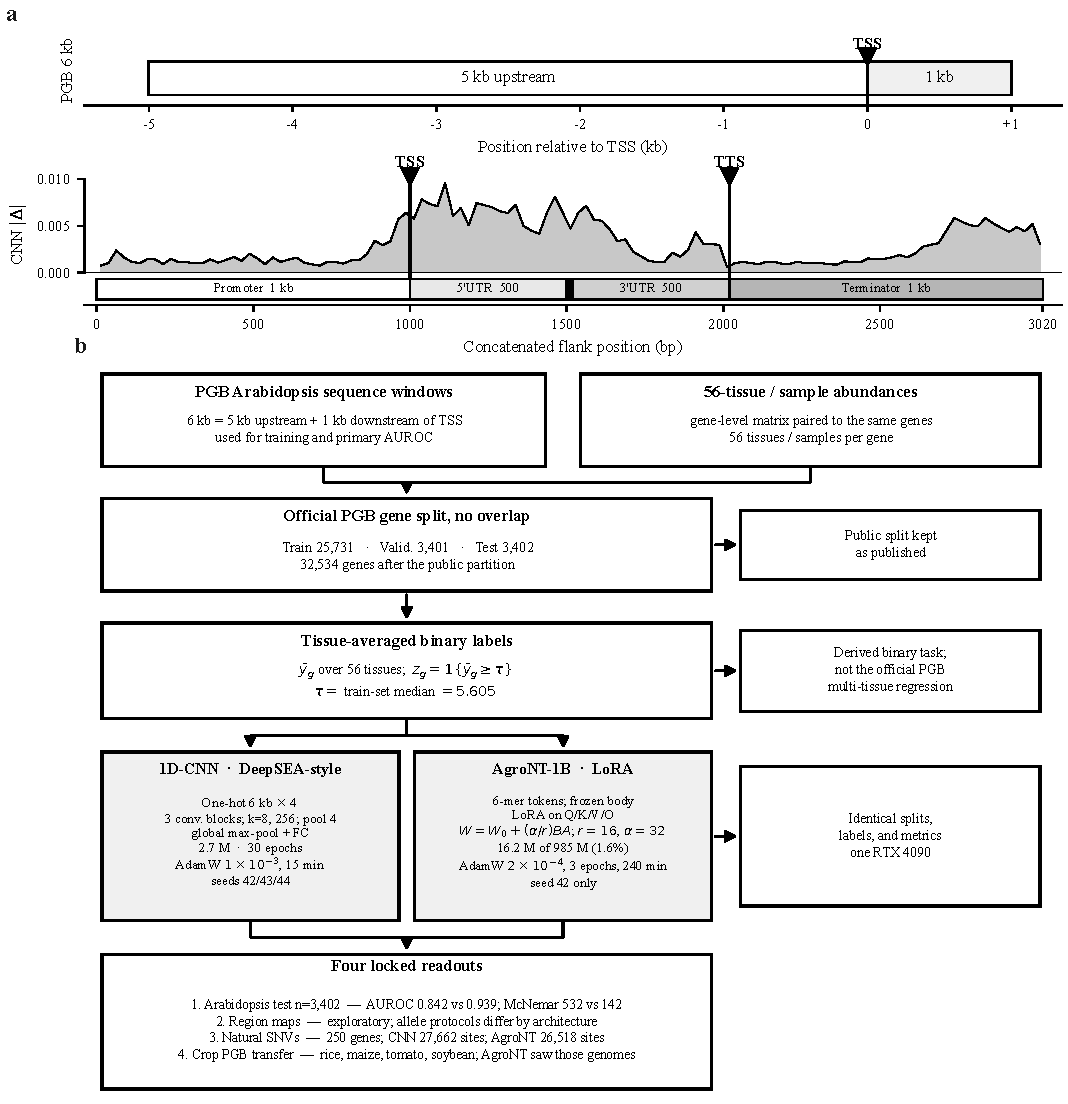
\includegraphics[width=\linewidth]{Figure1.pdf}
\caption{Locked evaluation protocol. PGB Arabidopsis 6~kb gene-centered windows and tissue-averaged high/low labels are scored by a DeepSEA-style 1D-CNN and by LoRA-tuned AgroNT-1B under identical splits and metrics. Readouts are the Arabidopsis held-out test, region importance, natural flanking single-nucleotide variants, and independent crop PGB test sets.}
\label{fig:protocol}
\end{figure}

\section{Materials and Methods}

\subsection{Data}

We used the \emph{Arabidopsis thaliana} gene-expression FASTA of the Plants Genomic Benchmark \citep{mendoza2024,pgb2024}. Each gene is represented by a 6-kb genomic window constructed as 5~kb upstream plus 1~kb downstream of the annotated transcription start site (TSS). Expression labels in the FASTA comprise 56 tissue/sample RNA-sequencing measurements. The official split comprises 25,731 training, 3,401 validation, and 3,402 test genes, with no gene overlap across splits. The official PGB gene-expression task is multi-tissue regression; here we derived binary high/low labels from the median of per-gene mean expression on the training set. Because labels aggregate expression across 56 tissues/samples, the benchmark targets sequence correlates of tissue-averaged abundance class, not organ-specific programs.

In parallel, we built a structured gene-centric dataset for region-level interpretability. For each of 27,436 protein-coding \emph{A.\ thaliana} genes with usable flanking annotation and expression (TAIR10/Araport11; Ensembl Plants release 59 \citep{agi2000,lamesch2012,harrison2024}), we extracted the promoter (1~kb upstream of the TSS), 5$'$UTR (500~nt), 3$'$UTR (500~nt), and terminator (1~kb downstream of the transcription termination site) in transcriptional orientation, concatenated the four regions 5$'\rightarrow$3$'$ with a 20-nt N-padding gap, and one-hot encoded the resulting 3,020-bp sequence. Genes were assigned to fixed chromosomal splits (train: chromosome 5, $n=6{,}331$; validation: chromosomes 3 and 4, $n=9{,}636$; test: chromosomes 1 and 2, $n=11{,}469$). Binary labels used the training-split median of $\log_2(\mathrm{mean\ expression}+1)$ (threshold 3.038).

\subsection{Model architectures}

\textbf{1D-CNN baseline.} We implemented a DeepSEA-style convolutional network \citep{zhou2015} with three convolutional blocks, each containing two 1D convolutions (256 filters, kernel size 8), batch normalization, ReLU activation, and max pooling (pool size 4), followed by global max pooling and two fully connected layers with dropout. The model has 2.7~M parameters.

\textbf{DNA foundation model.} AgroNT-1B \citep{mendoza2024} is a transformer of 985~M parameters pretrained on $\sim$10.5 million sequences from 48 edible plant genomes. We adapted it for sequence classification with LoRA adapters \citep{hu2021lora} (rank 16, $\alpha=32$) on the query/key/value/output projections of every self-attention block, plus a two-layer head over mean-pooled hidden states. Only the 16.2~M LoRA and head parameters (1.6\% of the total) were trainable.

\subsection{Training, interpretability, tissue labels, and variants}

Both models were trained with cross-entropy loss and early stopping on validation area under the receiver operating characteristic curve (AUROC). The CNN used batch size 64 and AdamW (learning rate $10^{-3}$) for up to 30 epochs. AgroNT used an effective batch size of 32 and AdamW (learning rate $2\times10^{-4}$) for up to 3 epochs, all on a single NVIDIA RTX 4090. Reported metrics were accuracy, AUROC, and area under the precision-recall curve (AUPRC). The PGB CNN was repeated with three seeds (42/43/44); AgroNT is reported from seed 42. An input-length ablation retrained both models after midpoint cropping of the 6~kb windows to 3~kb and 1.5~kb. Because that window is 5~kb upstream plus 1~kb downstream of the TSS, midpoint cropping removes most TSS-proximal sequence.

Matched region importance used sliding-window mutagenesis on structured flanking sequences (50-bp N substitution, 25-bp step). The CNN for this analysis was retrained on the concatenated flanking set (test AUROC 0.805). AgroNT mutagenesis applied the Arabidopsis PGB LoRA checkpoint to the same concatenated strings without retraining on that representation. DeepLift attributions \citep{shrikumar2017} on structured test genes supported TF-MoDISco-lite \citep{shrikumar2018} and TOMTOM annotation against JASPAR 2024 \citep{rauluseviciute2024}. Architecture comparisons of region ranks use the matched mutagenesis scores rather than DeepLift magnitudes.

We parsed the 56 tissue/sample values in PGB FASTA headers for 32,534 unique Arabidopsis genes and computed pairwise Spearman correlations, per-gene cross-tissue coefficient of variation (CV), and agreement between the tissue-averaged high/low label and each tissue's own median-based label (Figure~\ref{fig:tissue}).

Natural single-nucleotide variants from the Ensembl Plants \emph{A.\ thaliana} variation VCF \citep{harrison2024} were mapped onto the structured flanking representation of 250 genes. The CNN scored 27,662 variants by substituting the mapped alternate allele. AgroNT scored 26,518 overlapping non-gap sites as the mean $|\Delta|$ over the three non-reference bases. Region ranks are compared within each model. An overlap of 17 reported expression quantitative trait locus (eQTL) associations was contrasted with the CNN genome-wide background.

\subsection{Independent crop PGB evaluation}

Frozen Arabidopsis CNN and AgroNT checkpoints were applied, without crop fine-tuning, to the official PGB test sets of rice (\emph{Oryza sativa}; $n=3{,}702$), maize (\emph{Zea mays}; $n=4{,}483$), tomato (\emph{Solanum lycopersicum}; $n=3{,}827$), and soybean (\emph{Glycine max}; $n=4{,}803$). Labels used each species' training-split median. These four test sets were not used to train or select the Arabidopsis models. AgroNT was pretrained on genomes that include these crops \citep{mendoza2024}, so the crop readout is adapter transfer on a multi-species backbone; the CNN never trained on crop genomes. The two readouts are therefore not interchangeable species-unseen tests. They do provide independent public sequence-and-label sets against which the Arabidopsis ranking can be checked.

\subsection{Statistical analysis}

The CNN--AgroNT difference used 500-fold bootstrap 95\% confidence intervals on the test set and McNemar's test on paired classifications. Region-wise variant $|\Delta|$ comparisons used two-sided Mann--Whitney tests. Because four region pairs were inspected within each architecture, the pairwise $p$-values are reported raw; File S1 includes the underlying per-variant scores so that readers can apply a correction of choice. Tissue-label concordance is a descriptive agreement rate, not a multiple-testing screen. Crop AUROC values are reported per species without pooling.

\subsection{Data availability}

No unique biological reagents were generated. Primary inputs are public: PGB Arabidopsis and crop gene-expression FASTA \citep{pgb2024}, TAIR10/Araport11 annotations, Ensembl Plants variation, and JASPAR 2024. File S1 contains the processed score tables used to generate the figures. Training and evaluation code is included with this submission. An archival deposit that mints a DOI (for example Zenodo) will be provided before acceptance; a working GitHub copy alone is not the archival record. Model checkpoints will be deposited with that archive.

\section{Results}

\subsection{AgroNT outperforms the CNN on a unified Arabidopsis benchmark}

On the held-out PGB test set ($n = 3{,}402$), AgroNT reached 86.8\% accuracy (AUROC 0.939, AUPRC 0.935), compared with 75.4\% accuracy (AUROC 0.842, AUPRC 0.835) for the CNN (Table~\ref{tab:bench}; Figure~\ref{fig:bench}). The AUROC difference of 0.097 had a bootstrap 95\% CI of 0.086--0.108. McNemar's test was $p = 6.7\times10^{-54}$: 532 genes were classified correctly by AgroNT and incorrectly by the CNN, versus 142 the reverse. Across three CNN seeds, test AUROC was $0.844\pm0.003$ and accuracy $76.3\pm0.9\%$, so the primary CNN result is not a single-run outlier. Single-tissue labels agreed with the tissue-averaged label for a mean of 92.1\% of genes (range 78.7--95.4\%; median tissue--tissue Spearman 0.851; Figure~\ref{fig:tissue}), which supports using an averaged binary label for this architecture comparison.

\begin{table}[htbp]
\centering
\caption{Unified benchmark on the PGB Arabidopsis held-out test set (primary seed 42; $n = 3{,}402$). $\Delta$AUROC $= 0.097$ (bootstrap 95\% CI 0.086--0.108). McNemar: 532 vs 142 discordant pairs, $p = 6.7\times10^{-54}$. CNN three-seed AUROC $0.844\pm0.003$. Training time on one RTX 4090: 15~min (CNN) vs 240~min (AgroNT LoRA).}
\label{tab:bench}
\begin{tabular}{lcccc}
\toprule
Model & Trainable params & Accuracy & AUROC (95\% CI) & AUPRC \\
\midrule
1D-CNN (DeepSEA-style) & 2.7 M & 75.4\% & 0.842 (0.829--0.855) & 0.835 \\
AgroNT-1B (LoRA) & 16.2 M of 985 M & 86.8\% & 0.939 (0.931--0.947) & 0.935 \\
\bottomrule
\end{tabular}
\end{table}

\begin{figure}[htbp]
\centering

\includegraphics[width=\linewidth]{Figure2.pdf}
\caption{Head-to-head comparison on the PGB Arabidopsis test set. (a) Accuracy, AUROC, and AUPRC (values in Table~\ref{tab:bench}). (b) AUROC versus trainable-parameter count, annotated with single-GPU training time. AgroNT is plotted at 16.2~M trainable parameters.}
\label{fig:bench}
\end{figure}

\subsection{Proximal flanks carry predictive signal; variant ranks are architecture-specific}

On the structured flanking set, matched mutagenesis ranked mean importance per base as 5$'$UTR (0.073) $>$ terminator (0.066) $>$ promoter (0.060) $>$ 3$'$UTR (0.057) for the CNN and promoter (0.558) $>$ 3$'$UTR (0.545) $>$ 5$'$UTR (0.501) $>$ terminator (0.483) for AgroNT (Figure~\ref{fig:region}a,b). Absolute mutagenesis scales are not comparable across architectures. DeepLift attributions used for motif discovery ranked 5$'$UTR (0.0088) $>$ 3$'$UTR (0.0081) $>$ promoter (0.0048) $>$ terminator (0.0038). TF-MoDISco recovered four positive and four negative patterns; TOMTOM against JASPAR 2024 mapped hits that include DOF-family factors (DOF1.5, DOF3.4/3.6, DOF5.1/5.8, CDF5), SPL8, NAC005, and AGL1. Because short DOF-like cores also appear among negative patterns, motif annotation is provisional.

CNN scoring of 27,662 natural flanking variants mapped median $|\Delta|$ as 5$'$UTR (0.00269; $n=2{,}542$) $>$ 3$'$UTR (0.00112; $n=4{,}148$) $>$ terminator (0.00058; $n=13{,}573$) $>$ promoter (0.00043; $n=7{,}399$). Pooled UTR variants exceeded terminator variants (Mann--Whitney $p = 4.3\times10^{-98}$) and promoter variants ($p = 1.4\times10^{-106}$); 5$'$UTR exceeded 3$'$UTR ($p = 1.2\times10^{-61}$). AgroNT median $|\Delta|$ on 26,518 overlapping sites ranked terminator (0.00202) $>$ 3$'$UTR (0.00118) $>$ 5$'$UTR (0.00085) $>$ promoter (0.00054) (Table~\ref{tab:var}; Figure~\ref{fig:region}c,d). Promoter was the least sensitive compartment in both variant maps. Attribution, mutagenesis, and variant ranks are not required to agree beyond that shared promoter-lowest pattern. An exploratory overlap of 17 reported eQTL variants was higher than the CNN background (0.00205 vs.\ 0.00065; Mann--Whitney $p = 0.041$).

\begin{table}[htbp]
\centering
\caption{Predicted $|\Delta|$ in high-expression probability by flanking region (250 genes). CNN: mapped alternate allele. AgroNT: mean over three non-reference bases. Absolute $|\Delta|$ is not compared across architectures because the allele protocol differs.}
\label{tab:var}
\begin{tabular}{lcccc}
\toprule
Region & $n$ (CNN) & CNN median $|\Delta|$ & $n$ (AgroNT) & AgroNT median $|\Delta|$ \\
\midrule
5$'$UTR & 2,542 & 0.00269 & 2,474 & 0.00085 \\
3$'$UTR & 4,148 & 0.00112 & 3,997 & 0.00118 \\
Terminator & 13,573 & 0.00058 & 12,958 & 0.00202 \\
Promoter & 7,399 & 0.00043 & 7,089 & 0.00054 \\
\bottomrule
\end{tabular}
\end{table}

\begin{figure}[htbp]
\centering
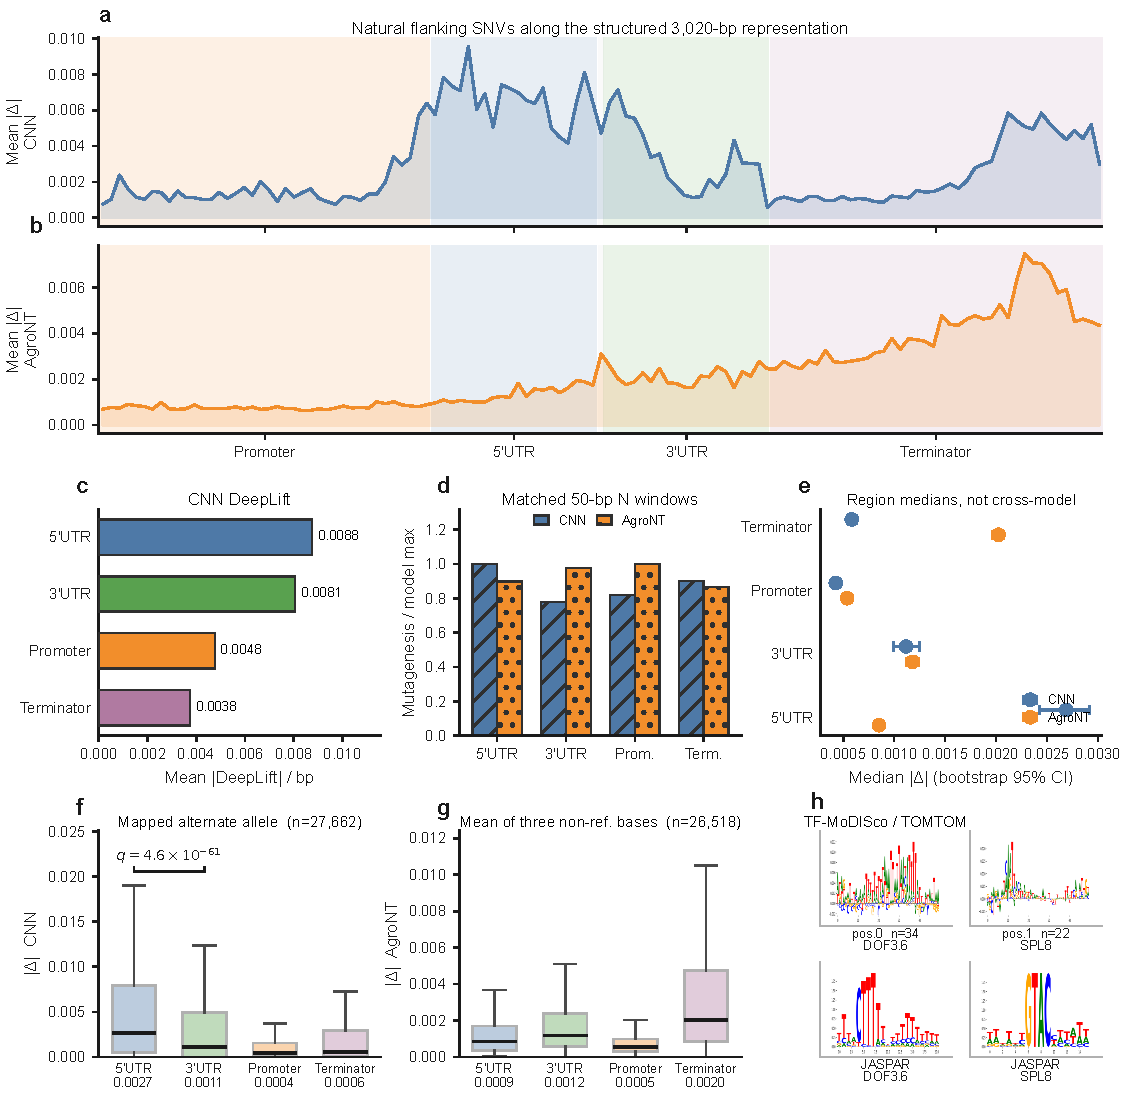
\includegraphics[width=\linewidth]{Figure3.pdf}
\caption{Region importance and variant effects on the structured flanking representation. (a) Mean absolute DeepLift attribution per base for the CNN. (b) Matched sliding-window mutagenesis for both models, normalized to each model's maximum. (c) CNN variant $|\Delta|$ by region (mapped alternate allele; 5$'$UTR vs 3$'$UTR Mann--Whitney $p = 1.2\times10^{-61}$). (d) AgroNT variant $|\Delta|$ at overlapping sites (mean over three non-reference bases).}
\label{fig:region}
\end{figure}

\subsection{The Arabidopsis ranking holds on independent crop PGB test sets}

On the four crop PGB test sets, which were never used for Arabidopsis training, the Arabidopsis-trained CNN reached AUROC 0.716 (rice), 0.685 (maize), 0.763 (tomato), and 0.759 (soybean). The same Arabidopsis AgroNT LoRA checkpoint reached 0.815, 0.894, 0.838, and 0.878 (Figure~\ref{fig:transfer}a,b). AgroNT remained ahead on every crop; the largest gap was maize. Crop AUROC was lower than Arabidopsis self-performance (CNN 0.842; AgroNT 0.939), as expected for a cross-species application of Arabidopsis checkpoints. Retraining after midpoint-cropping the 6~kb windows to 3~kb or 1.5~kb gave CNN AUROC 0.542 and 0.545 and AgroNT AUROC 0.625 and 0.580 (Figure~\ref{fig:transfer}c). Under the TSS-anchored 5~kb+1~kb geometry, midpoint cropping removes most TSS-proximal sequence, so that series tests this window geometry rather than gene-body centering. The structured 3,020-bp flanking representation, which keeps complete annotated proximal flanks, reached CNN test AUROC 0.805 on its chromosomal split; that number is not pooled with the PGB truncation series because split and sequence layout differ.

\begin{figure}[htbp]
\centering

\includegraphics[width=\linewidth]{Figure4.pdf}
\caption{Independent crop PGB evaluation and window geometry. (a) Arabidopsis-trained CNN applied to rice, maize, tomato, and soybean PGB test sets under each species' training-set median labels. (b) The same protocol for the Arabidopsis AgroNT LoRA checkpoint. (c) Test AUROC after retraining both models on midpoint-cropped 6~kb, 3~kb, and 1.5~kb PGB windows.}
\label{fig:transfer}
\end{figure}

\section{Discussion}

The contest this study is built to win is a locked-protocol comparison: LoRA-tuned AgroNT versus a DeepSEA-style 1D-CNN on tissue-averaged Arabidopsis PGB labels. Under that protocol the AUROC gain is 0.097 (bootstrap 95\% CI 0.086--0.108; McNemar $p = 6.7\times10^{-54}$). The direction agrees with AgroNT's published PGB suite \citep{mendoza2024}. LoRA trains 1.6\% of AgroNT parameters. When a $\sim$0.1 AUROC improvement on this binary task is the decision criterion, the LoRA checkpoint is the stronger of the two models reported here; when a 2.7~M-parameter network is the operating constraint, the CNN is the compact baseline in the same table. The comparison is defined against this DeepSEA-style architecture, not against plant-specific flanking CNNs that can exceed 80\% accuracy on other high/low datasets \citep{peleke2024}.

On the structured representation, matched mutagenesis and DeepLift both place predictive importance in proximal annotated flanks. CNN DeepLift and CNN mutagenesis agree that the 5$'$UTR is among the strongest compartments, consistent in direction with prior reports that UTR sequence contributes to plant expression prediction \citep{peleke2024}. This is a predictive association with tissue-averaged mRNA-abundance class. Variant $|\Delta|$ ranks UTR $>$ terminator $>$ promoter for this CNN and terminator $>$ UTR $>$ promoter for AgroNT; promoter is the shared least-sensitive compartment. Attribution, mutagenesis, and variant maps are not a causal cis-regulatory atlas.

High tissue--tissue correlation and 92.1\% mean label concordance support the averaged binary benchmark for architecture comparison. Concordance as low as 78.7\% is the scope condition for organ-specific programs, which remain a tissue-conditioned task \citep{peleke2024}. Independent crop PGB test sets keep the same model ranking (CNN AUROC 0.685--0.763; AgroNT 0.815--0.894). Those sets were not used in Arabidopsis training. The two crop readouts are still not the same experiment: the CNN never saw crop genomes, whereas AgroNT's backbone already included those species in pretraining. Midpoint cropping of the published 6~kb window is tied to this TSS-anchored geometry for both architectures.

The evaluation is defined for tissue-averaged Arabidopsis PGB labels, a TSS-anchored 6~kb window, LoRA training of at most three epochs, and a single AgroNT seed. DeepLift motif discovery was run on the CNN; AgroNT mutagenesis used the PGB LoRA checkpoint on concatenated flanks without retraining on that representation; variant $|\Delta|$ used mapped alleles for the CNN and three-alt means for AgroNT on 250 genes; the eQTL overlap used $n=17$ associations; structured UTR lengths are fixed at 500~nt. Tissue-of-expression labels, accessibility or methylation \citep{omalley2016,takou2025}, larger eQTL sets, and longer-context DNA language models \citep{avsec2021} are outside this protocol.

\section{Conclusions}

On a derived Arabidopsis PGB task with tissue-averaged labels, LoRA-tuned AgroNT outperforms this DeepSEA-style 1D-CNN by a statistically supported margin under the reported budgets. Predictive importance concentrates in proximal annotated flanks. CNN variant $|\Delta|$ is led by the 5$'$UTR and AgroNT variant $|\Delta|$ by the terminator; both maps leave the promoter lowest. Tissue-averaged labels align with most single-tissue binary axes. The same Arabidopsis checkpoints keep that ranking on independent rice, maize, tomato, and soybean PGB test sets.

\section*{Data availability}

Primary inputs are public: PGB Arabidopsis and crop gene-expression FASTA \citep{pgb2024}, TAIR10/Araport11 annotations, Ensembl Plants variation, and JASPAR 2024. File S1 contains processed score tables used for the figures. Training and evaluation code is included with this submission. An archival repository that issues a DOI will be named before acceptance; model checkpoints will be deposited with that archive.

\section*{Acknowledgments}

None.

\section*{Funding}

This research received no external funding.

\section*{Conflicts of interest}

The authors declare no conflicts of interest.

\section*{Author contributions}

To be completed before submission (CRediT). All authors will approve the final version and accept responsibility for accuracy.

\clearpage
\section*{Supplemental material}

\setcounter{figure}{0}
\renewcommand{\thefigure}{S\arabic{figure}}

\begin{figure}[htbp]
\centering
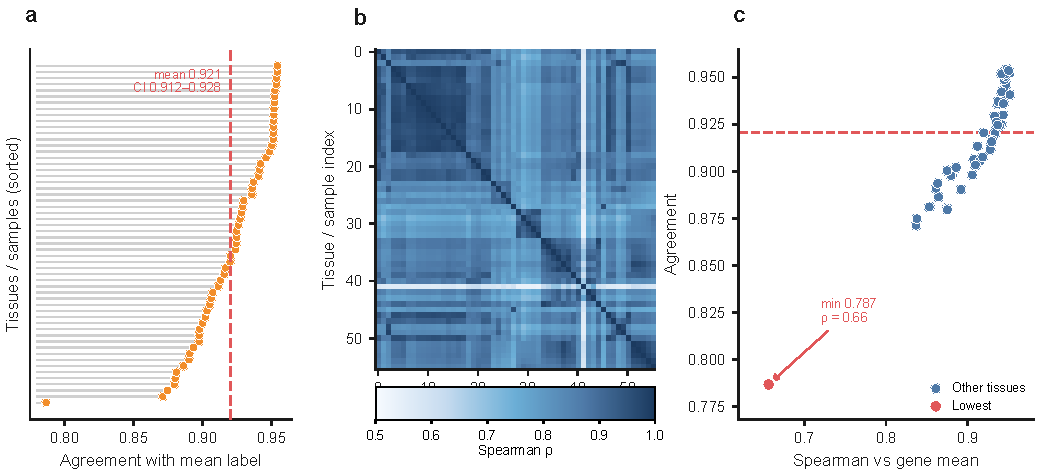
\includegraphics[width=\linewidth]{FigureS1.pdf}
\caption{Scope of tissue-averaged labels across 32,534 genes and 56 tissues/samples. (a) Concordance of each tissue's median-based high/low label with the tissue-averaged label (mean agreement 0.921). (b) Pairwise Spearman correlation among tissues. Cross-tissue CV: median 0.340, 75th percentile 1.37. File S1 contains the processed tables underlying this figure and the main tables.}
\label{fig:tissue}
\end{figure}

\bibliography{refs}

\end{document}
